\section{Introduction} \label{sec:intro}



\paragraph{Markov Models}
A Markov Model is a class of model where the system being studied undergoes random and independent state changes. Markov Models are said to obey the ``Markov Property,'' that is, the probability of the system changing states is dependent only on the current state of the system, and not on any previous states. That is to say 
    \begin{align*}
      P[q_t &= S_i | q_{t-1} = S_i, q_{t-2} = S_k, ...]\\
      &= P[q_t = S_i | q_{t-1} = S_i]
    \end{align*}
where $q_t$ is the state of the system at time $t$ and $S_i$ is the $i$th possible state for the system. This memorylessness gives Markov Models some very nice properties for proabilistic analysis that allows for efficient modeling of otherwise very computationally intensive systems. Many important systems of study also follow the Markov Property by nature, such as the Brownian Motion of atoms or the dynamics or allele frequencies in a population. 

\paragraph{Hidden Markov Models}
Here we look at one variant of Markov Models, the so-called Hidden Markov Models or HMMs. These HMMs are considered ``Hidden'' because the system's state cannot be observed at any time. Instead, at each timestep, the system emits one of several possible observations $O_i$. Each state has its own probability distribution for which observation to emit. (Note: continuous time Hidden Markov Models do exist, but we restrict our analysis to discrete time variants). 

The structure of a Hidden Markov Model is composed of two matrices: one that holds the state change transition probabilities, and one that holds the emission probabilities of each of the obseravations for each state. A HMM must also have a probability distribution for selecting a starting state $\pi$ \[
  \pi_i = P[q_1 = S_i], \ \ \ 1 \leq i \leq N.
\] For a concrete example, we'll look at a student's course selection at a hypothetical college. This is a very small school, with only three departments: computer science, biology, and linguistics. Our student starts out as a major in one of these three departments with probability \[
  \pi = \begin{cases} 
            0.5 & \text{Computer Science}\\
            0.3 & \text{Biology}\\
            0.2 & \text{Linguistics}
          \end{cases}
\] She will change majors at each semester according to the state transition matrix \[
  A = \{a_{ij}\} = \begin{bmatrix}
                      0.8 & 0.1 & 0.1\\
                      0.2 & 0.7 & 0.1\\
                      0.1 & 0.3 & 0.6
                    \end{bmatrix}
\] Students at this school do not tell their major to anyone. Instead, one has to guess their major by asking their plans after graduation. Every student says they either want to go to medical school, graduate school, law school, or find a job right away. The probabilities of saying any of these options depends on their current major according to the observation matrix \[
  B = P[v_k \text{ at } t|q_t = S_j] = \begin{bmatrix}
                                        0.05 & .4 & 0.05 & 0.5\\
                                        0.8 & 0.1 & 0.05 & 0.05\\
                                        0 & 0.95 & 0.05 & 0
                                      \end{bmatrix}
\] With $1 \leq j \leq N, 1 \leq k \leq M$. (Note: $B$ is often represented as a function $b_j(k) = P[v_k \text{ at } t|q_t = S_j]$, but we represent it as a matrix and implement it as such). 


\tikzset{statenode/.style={circle, draw, very thick, minimum size=20mm}}
\tikzset{observnode/.style={rectangle, draw, very thick, minimum size=20mm}}
%\tikzset{loop/.style={looseness=10}}
\begin{figure}
	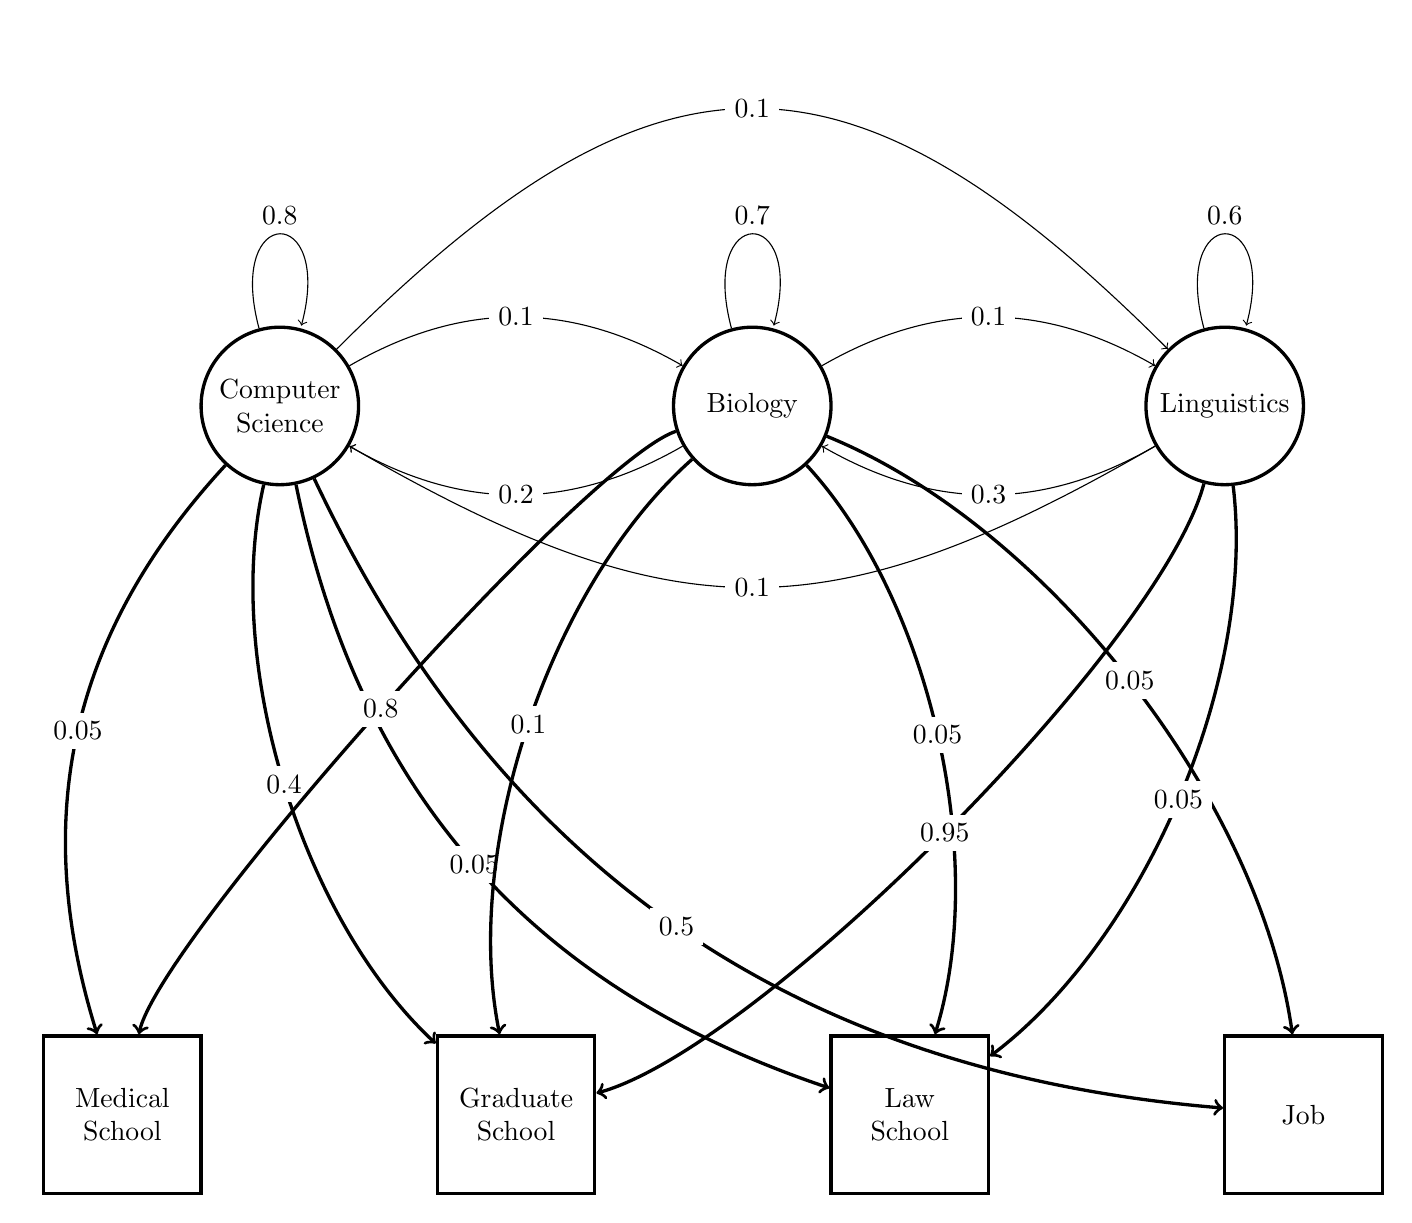
\begin{tikzpicture}
		%states
		\node[statenode] (CS) at (2,0) [draw, align=center] {Computer \\ Science};
		\node[statenode] (bio) at (8,0) {Biology};
		\node[statenode] (ling) at (14, 0) {Linguistics};


		%transition probabilities
		 \path[->] (CS) edge  [loop above] node {0.8} ();
		 \path[->] (CS) edge [bend left] node [fill=white] {0.1} (bio);
		 \path[->] (CS) edge [looseness = 1.4] node [fill=white] {0.1} (ling);

		 \path[->] (bio) edge [bend left] node [fill=white] {0.2} (CS);
		 \path[->] (bio) edge [loop above] node {0.7} ();
		 \path[->] (bio) edge [bend left] node [fill=white] {0.1} (ling);


		 \path[->] (ling) edge [bend left, looseness = 1.2] node [fill=white] {0.1} (CS);
		 \path[->] (ling) edge [bend left] node [fill=white] {0.3} (bio);
		 \path[->] (ling) edge [loop above] node {0.6} ();



		 %emission probabilities
		 \node[observnode] (med) at (0, -9) [draw, align=center] {Medical \\ School};
		 \node[observnode] (grad) at (5, -9) [draw, align=center] {Graduate \\ School};
		 \node[observnode] (law) at (10, -9) [draw, align=center] {Law \\ School};
		 \node[observnode] (job) at (15, -9) [draw, align=center] {Job};

		 \path[->, very thick] (CS) edge [bend right] node [fill=white] {0.05} (med);
		 \path[->, very thick] (CS) edge [bend right, looseness = 0.8] node [fill=white] {0.4} (grad);
		 \path[->, very thick] (CS) edge [bend right] node [fill=white, looseness = 0.6] {0.05} (law);
		 \path[->, very thick] (CS) edge [bend right] node [fill=white, looseness = 0.4] {0.5} (job);


		\path[->, very thick] (bio) edge [bend right, looseness = 0.3] node [fill=white] {0.8} (med);
		\path[->, very thick] (bio) edge [bend right, looseness = 0.8] node [fill=white] {0.1} (grad);
		\path[->, very thick] (bio) edge [bend left, looseness = 0.8] node [fill=white] {0.05} (law);
		\path[->, very thick] (bio) edge [bend left, looseness = 0.8] node [fill=white] {0.05} (job);



		\path[->, very thick] (ling) edge [bend left, looseness = 0.5] node [fill=white] {0.95} (grad);
		\path[->, very thick] (ling) edge [bend left, looseness = 0.8] node [fill=white] {0.05} (law);



	\end{tikzpicture}
	Figure 1. A Trellis diagram for the Hidden Markov Model example outlined in the introduction. Circles are possible states and squares are possible observations. Thin line represent state change probabilities and thick lines represent emission probabilities. 
\end{figure}

\paragraph{Motivation and Applications}
Hidden Markov Models are extremely useful for modeling complex probabilistic processes in the real world. The above example may not be terribly realistic, but that's mostly because it is simplified for illustration purposes (I'm sure some linguistics majors can find jobs). HMMs become useful when systems grow to be increasingly complex, and analyses that cannot assume independence of events become computationally intractable. 

HMMs have many applications in bioinformatics, especially in computational genome annotation. Many algorithms exist to iterate a newly assembled genome and attempt to determine the state of each segment of DNA as one of the possible genome elements (i.e. exon, intron, non-coding region, ...). The true state of each position is unknown, and model parameters can only be estimated. Because of the large size of genomes, this is one example of when the relative computational simplicity of HMMs is very beneficial. 

Moreover, HMMs are used heavily in computational linguistics both for audio speech recognition and part-of-speech recognition. Audio signals can be discretized by taking short segments (i.e. 10 milliseconds) and looking at the most significant coefficients from the Fourier transform. In this way, a HMM can be trained to identify the discrete phonemes of a spoken language with a high degree of accuracy and little training time. Higher-order HMMs can then identify which part of speech a given word is most likely to be given what part of speech the previous word is.

Once processes are modeled as HMMs, one can clearly see the motivation behind calculating certain properties, such as the most likely sequence of states, or how to find unknown model parameters. In the following sections, we will provide algorithms for determining these properties.